% ============================================================
%  Entrega Final — Predicción de Churn en E-commerce (Olist)
%  Archivo único — máximo 10 páginas de reporte
% ============================================================
\documentclass[11pt]{article}

\usepackage[margin=0.9in]{geometry}
\usepackage[T1]{fontenc}
\usepackage[utf8]{inputenc}
\usepackage{lmodern}
\usepackage{microtype}
\usepackage{amsmath}
\usepackage{graphicx}
\usepackage{float}
\usepackage{booktabs}
\usepackage{array}
\usepackage{tabularx}
\usepackage{caption}
\usepackage{subcaption}
\usepackage{ragged2e}
\usepackage{enumitem}
\usepackage{hyperref}
\hypersetup{colorlinks=true,linkcolor=blue,urlcolor=blue}

\setlength{\parskip}{4pt}

\title{Entrega Final --- Predicción de Churn en E-commerce (Olist)\\
\large Modelos, API, Tablero React/Vite y Despliegue en AWS EC2}
\author{
David Alan Delgado Zarco \and
Octavio Esquivel Alvarez del Castillo \and
John Williams Morrill \and
Jason Rosher Morrill
}
\date{Marzo 10, 2026}

\begin{document}
\maketitle

% ============================================================
\begin{abstract}
Se presenta el producto final de predicción de churn para clientes del dataset
Olist con ventana $W{=}90$ días. El label se construye sin data leakage usando
una arquitectura de ventana temporal (snapshot + ventana futura). Se entrenan y
comparan Regresión Logística y Random Forest, evaluados con PR-AUC para la
clase no-churn. Los experimentos se registran en MLflow desplegado en AWS EC2.
Como producto final se entrega un tablero React/Vite servido por una API Express
(Node.js + Python joblib) y desplegado en EC2 con PM2, que permite estimar la
probabilidad de churn de un cliente junto con la contribución interpretable de cada feature.
\end{abstract}

% ============================================================
\section{Resumen del problema}

\paragraph{Contexto.}
Olist es un marketplace brasileño que conecta vendedores con clientes a través
de múltiples canales. El historial de transacciones muestra que la gran mayoría
de los compradores realiza una sola compra, generando un fuerte desbalance entre
clientes que regresan (no-churn) y los que no vuelven (churn). Retener un
comprador recurrente tiene un valor económico significativamente mayor que
adquirir uno nuevo, por lo que identificar de forma temprana a los clientes en
riesgo es una prioridad operativa.

\paragraph{Pregunta de negocio y alcance.}
\textit{¿Es posible anticipar, a partir del historial transaccional y de
experiencia de un cliente, si volverá a comprar en los próximos 90 días?}
El alcance incluye: (i)~definición rigurosa del label sin leakage, (ii)~pipeline
de features a nivel cliente, (iii)~modelo supervisado desplegado en una API, y
(iv)~tablero interactivo accesible en la nube.

\paragraph{Datos.}
Se utilizaron cinco archivos del dataset público de Olist: \texttt{orders},
\texttt{customers}, \texttt{payments}, \texttt{reviews} e \texttt{items}. Cada
tabla 1:N se agrega por \texttt{order\_id} antes del join para evitar duplicación
de registros. El dataset final contiene clientes activos con al menos una compra
en un lookback de 180 días previo al snapshot.

\paragraph{Cambios respecto a la Entrega 2.}
\begin{itemize}[itemsep=1pt, topsep=2pt]
  \item El tablero migró de Streamlit a \textbf{React/Vite + API Express (Node.js)},
        con predicción en tiempo real y panel de contribución de features.
  \item La inferencia se sirve vía \texttt{POST /api/predict} usando el modelo
        \texttt{.joblib} invocado desde Python como proceso hijo (\texttt{spawn}).
  \item El despliegue se automatizó con \texttt{deploy\_churn\_dashboard.sh} y
        se gestiona con PM2 en EC2 (puerto 3000).
  \item El reporte incorpora métricas con umbral ajustado ($\hat{\tau}=0.12$) y
        manuales de usuario e instalación.
\end{itemize}

% ============================================================
\section{Datos y construcción del label}

\subsection*{Construcción del label sin leakage}

Se define una \textbf{fecha de snapshot} y una \textbf{ventana futura} $W=90$
días. El churn se asigna observando compras exclusivamente en el período
posterior:
\[
  \text{churn}=1 \iff \text{el cliente no compra en }
  (\textit{snapshot},\; \textit{snapshot}+90\text{ días}]
\]
$\text{churn}=0$ (no-churn / recompra) si el cliente sí compra dentro de la
ventana. La población se restringe a clientes con al menos una compra en el
lookback de 180 días previo al snapshot, evitando incluir clientes
históricamente inactivos. Se verificó que no existan duplicados por
\texttt{order\_id} (duplicados\,=\,0), garantizando integridad en los agrupados.

% ============================================================
\section{Features y partición temporal}

\subsection*{Features a nivel \texttt{customer\_unique\_id}}

\begin{itemize}[itemsep=1pt, topsep=2pt]
  \item \textbf{RFM:} \textit{Recency} (días desde última compra hasta snapshot),
        \textit{Frequency} (órdenes únicas), \textit{Monetary} (suma de pagos).
  \item \textbf{Experiencia / logística:} promedio de review score, días de
        entrega, días de retraso vs.\ fecha estimada, número de ítems, suma de
        precio y suma de flete.
  \item \textbf{Contexto geográfico:} \texttt{customer\_state} (one-hot encoding,
        \texttt{handle\_unknown="ignore"}).
\end{itemize}

\subsection*{Partición temporal}

Para evitar \textit{data leakage} se ordenan los clientes por su última compra
previa al snapshot y se separan por percentil 80: el 80\,\% más antiguo forma el
conjunto de entrenamiento y el 20\,\% más reciente el de prueba. Esto simula un
escenario de producción donde el modelo se evalúa en clientes cuyo futuro aún no
se conoce.

% ============================================================
\section{Modelos y evaluación}

\subsection*{Baseline y desbalance}

El dataset presenta fuerte desbalance: la clase minoritaria es el no-churn
(recompra). Un clasificador trivial que prediga siempre churn alcanza alta
accuracy pero obtiene $F_1^{(0)}=0$, lo que motiva el uso de métricas
enfocadas en la clase de interés.

\subsection*{Modelos comparados}

Se entrenaron dos pipelines con preprocesamiento idéntico
(imputación mediana + escala estándar para numéricas; imputación moda +
one-hot para categóricas):

\begin{itemize}[itemsep=1pt, topsep=2pt]
  \item \textbf{Regresión Logística}: \texttt{class\_weight=balanced},
        \texttt{C=0.1}, \texttt{max\_iter=2000}.
  \item \textbf{Random Forest}: \texttt{class\_weight=balanced\_subsample},
        \texttt{n\_estimators=400}.
\end{itemize}

\subsection*{Métricas y selección de umbral}

La métrica principal es el \textbf{PR-AUC para no-churn}
(\texttt{pr\_auc\_nochurn\_0}). Se realizó un barrido de 99 umbrales para
la Regresión Logística, seleccionando $\hat{\tau}=0.12$ como el valor que
maximiza $F_1^{(0)}$.

\begin{table}[H]
\centering
\caption{Comparación de modelos (umbral 0.5 para comparación directa; LogReg con
$\hat{\tau}=0.12$ en la última fila).}
\small
\begin{tabular}{lcccccc}
\toprule
\textbf{Modelo} & \textbf{Acc.} & \textbf{F1\,(churn)} &
\textbf{Prec.\,(no-ch.)} & \textbf{Rec.\,(no-ch.)} &
\textbf{F1\,(no-ch.)} & \textbf{PR-AUC\,(no-ch.)} \\
\midrule
Baseline (todo churn)   & alto  & alto & 0.000 & 0.000 & 0.000 & — \\
Random Forest           & 0.989 & 0.994 & 0.000 & 0.000 & 0.000 & 0.014 \\
LogReg ($\tau=0.50$)    & 0.467 & 0.633 & 0.013 & 0.613 & 0.025 & 0.035 \\
\textbf{LogReg ($\hat\tau=0.12$)} & — & — & — & — & \textbf{0.113} & \textbf{0.035} \\
\bottomrule
\end{tabular}
\end{table}

La Regresión Logística supera al Random Forest en PR-AUC para no-churn
(0.035 vs.\ 0.014) y es el único modelo que detecta la clase minoritaria de
forma no trivial. El umbral ajustado a $0.12$ eleva $F_1^{(0)}$ de 0.025 a
0.113. El run ganador en MLflow es \texttt{logreg\_C0.1\_thr012}.

\begin{figure}[H]
\centering
\begin{subfigure}[b]{0.46\textwidth}
  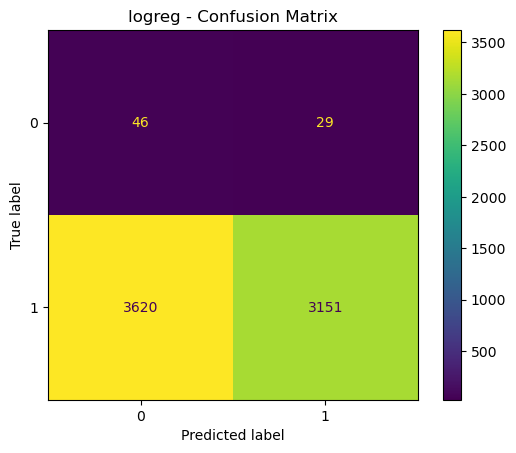
\includegraphics[width=\textwidth]{evidence/model/FIG_MODEL_01_cm_logreg.png}
  \caption{Matriz de confusión — LogReg ($\hat\tau=0.12$).}
\end{subfigure}
\hfill
\begin{subfigure}[b]{0.46\textwidth}
  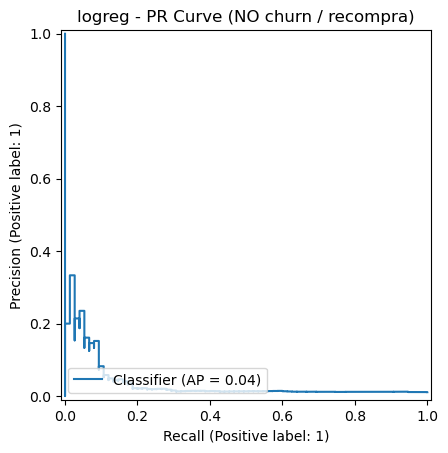
\includegraphics[width=\textwidth]{evidence/model/FIG_MODEL_02_pr_logreg.png}
  \caption{Curva PR para no-churn — LogReg.}
\end{subfigure}
\caption{Evaluación del modelo ganador.}
\end{figure}

% ============================================================
\section{Soportes en MLflow (AWS EC2)}

MLflow Tracking Server se desplegó en una instancia \textbf{EC2 Ubuntu}
(puerto 5000, backend SQLite, artefactos en \texttt{/home/ubuntu/mlruns}).
Se documentan evidencias con IP pública y usuario.
Repositorio: \url{https://github.com/Jason-Morrill/Microproyecto_proyectogrado}

\begin{figure}[H]
\centering
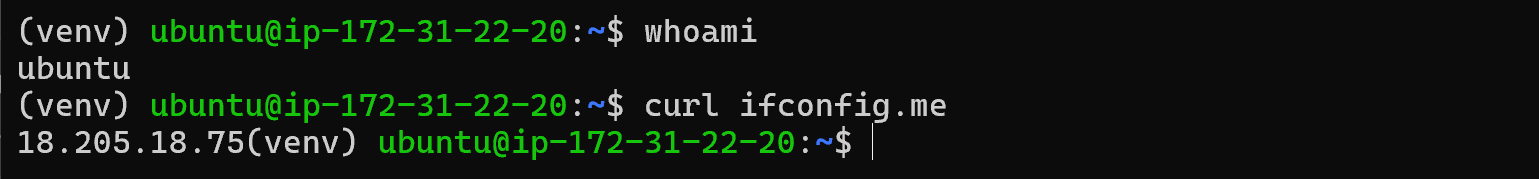
\includegraphics[width=0.7\textwidth]{evidence/aws/EVID_AWS_01_ec2_whoami_ip.png}
\caption{EC2: usuario e IP pública.}
\end{figure}

\begin{figure}[H]
\centering
\begin{subfigure}[b]{0.48\textwidth}
  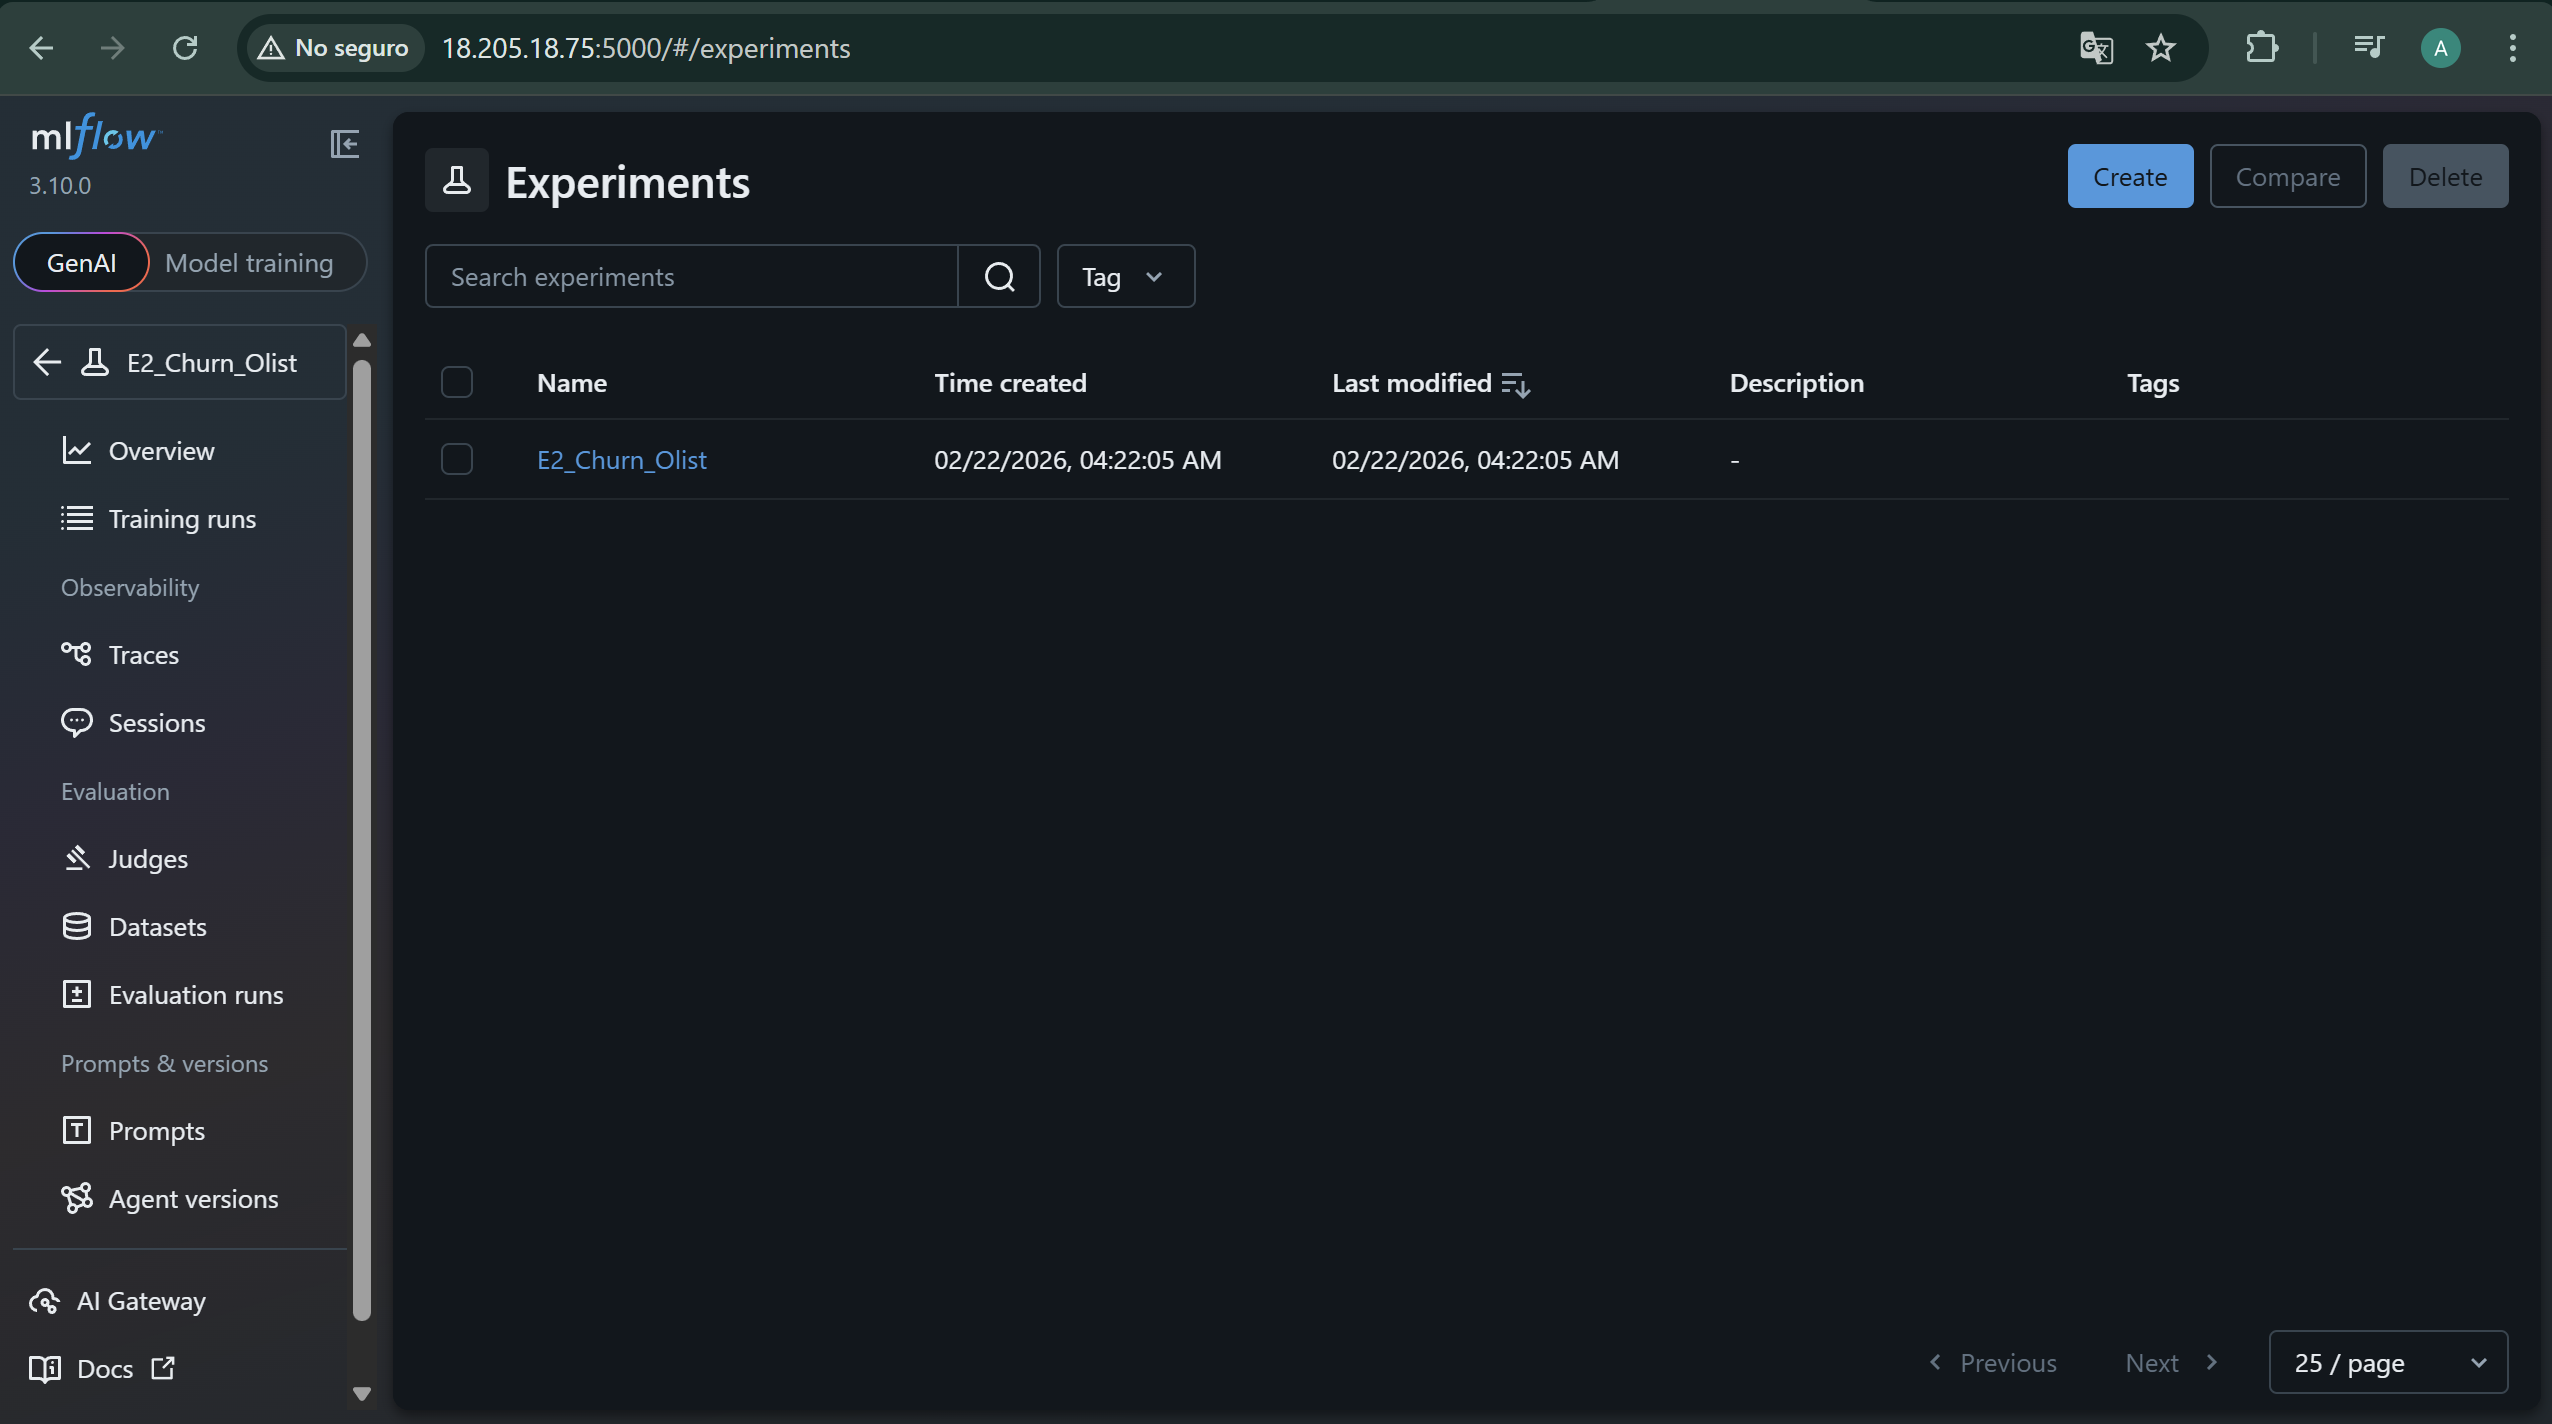
\includegraphics[width=\textwidth]{evidence/mlflow/EVID_MLFLOW_01_ui_ip.png}
  \caption{UI MLflow con IP pública.}
\end{subfigure}
\hfill
\begin{subfigure}[b]{0.48\textwidth}
  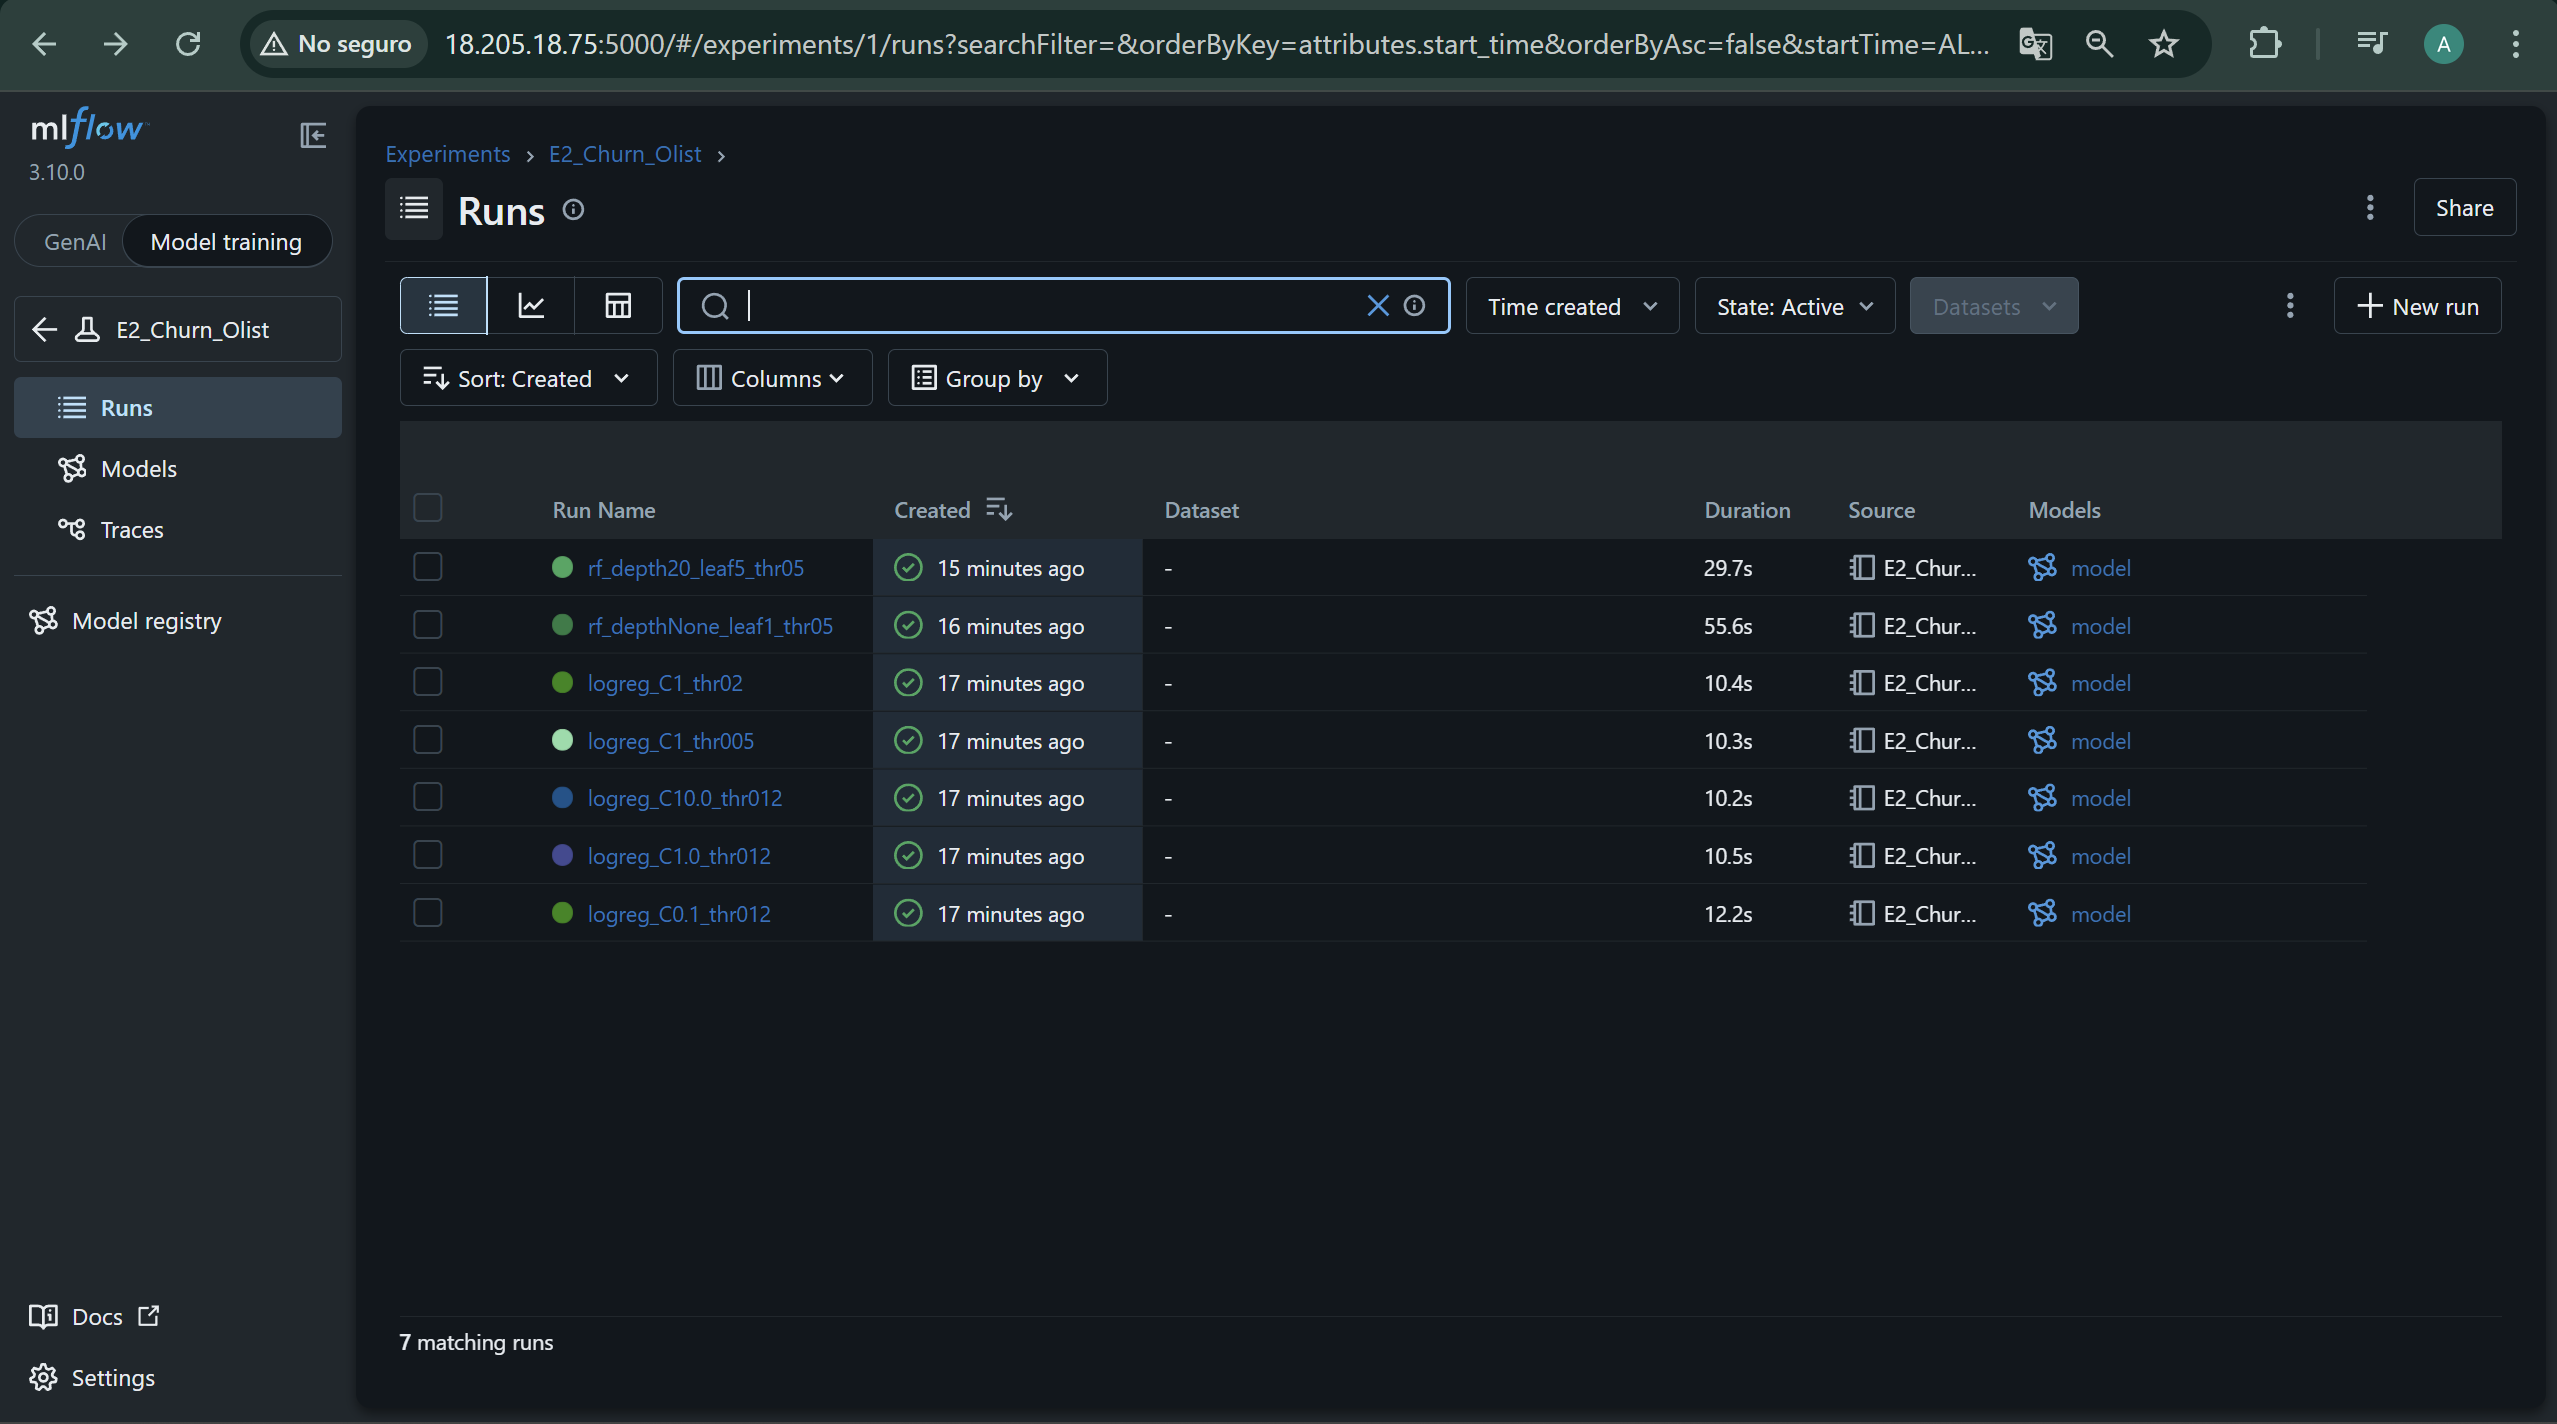
\includegraphics[width=\textwidth]{evidence/mlflow/EVID_MLFLOW_02_runs_list.png}
  \caption{Lista de runs del experimento.}
\end{subfigure}
\caption{MLflow: acceso y experimentos.}
\end{figure}

\begin{figure}[H]
\centering
\begin{subfigure}[b]{0.48\textwidth}
  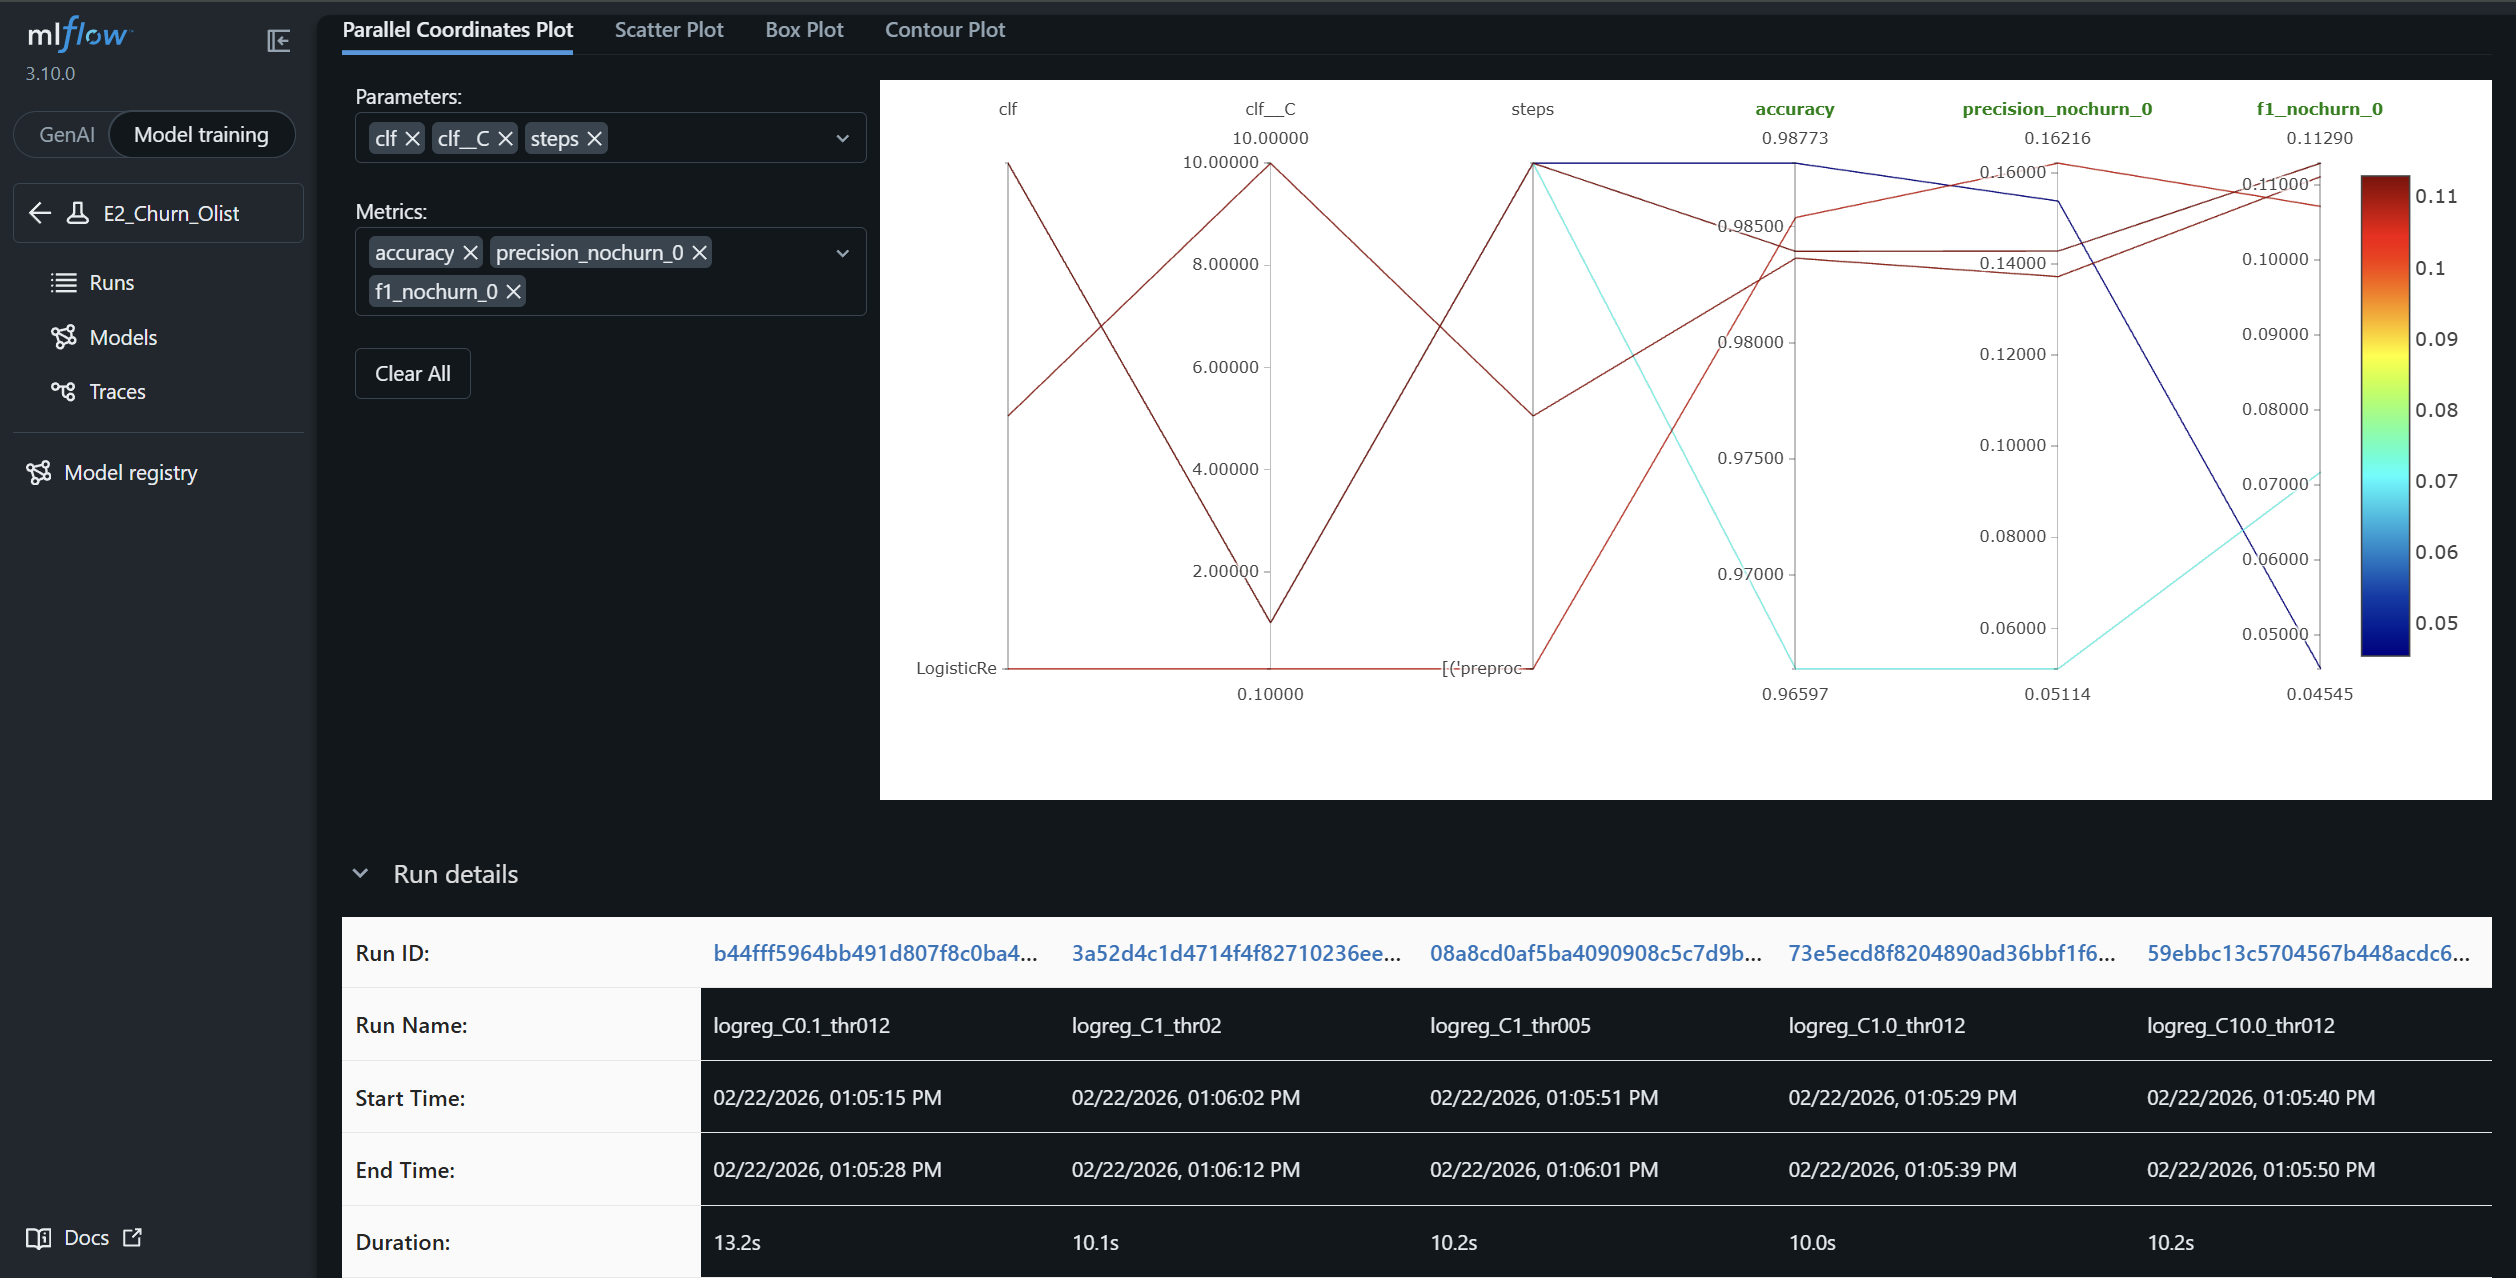
\includegraphics[width=\textwidth]{evidence/mlflow/EVID_MLFLOW_03_compare.png}
  \caption{Comparación de runs (\texttt{pr\_auc\_nochurn\_0}).}
\end{subfigure}
\hfill
\begin{subfigure}[b]{0.48\textwidth}
  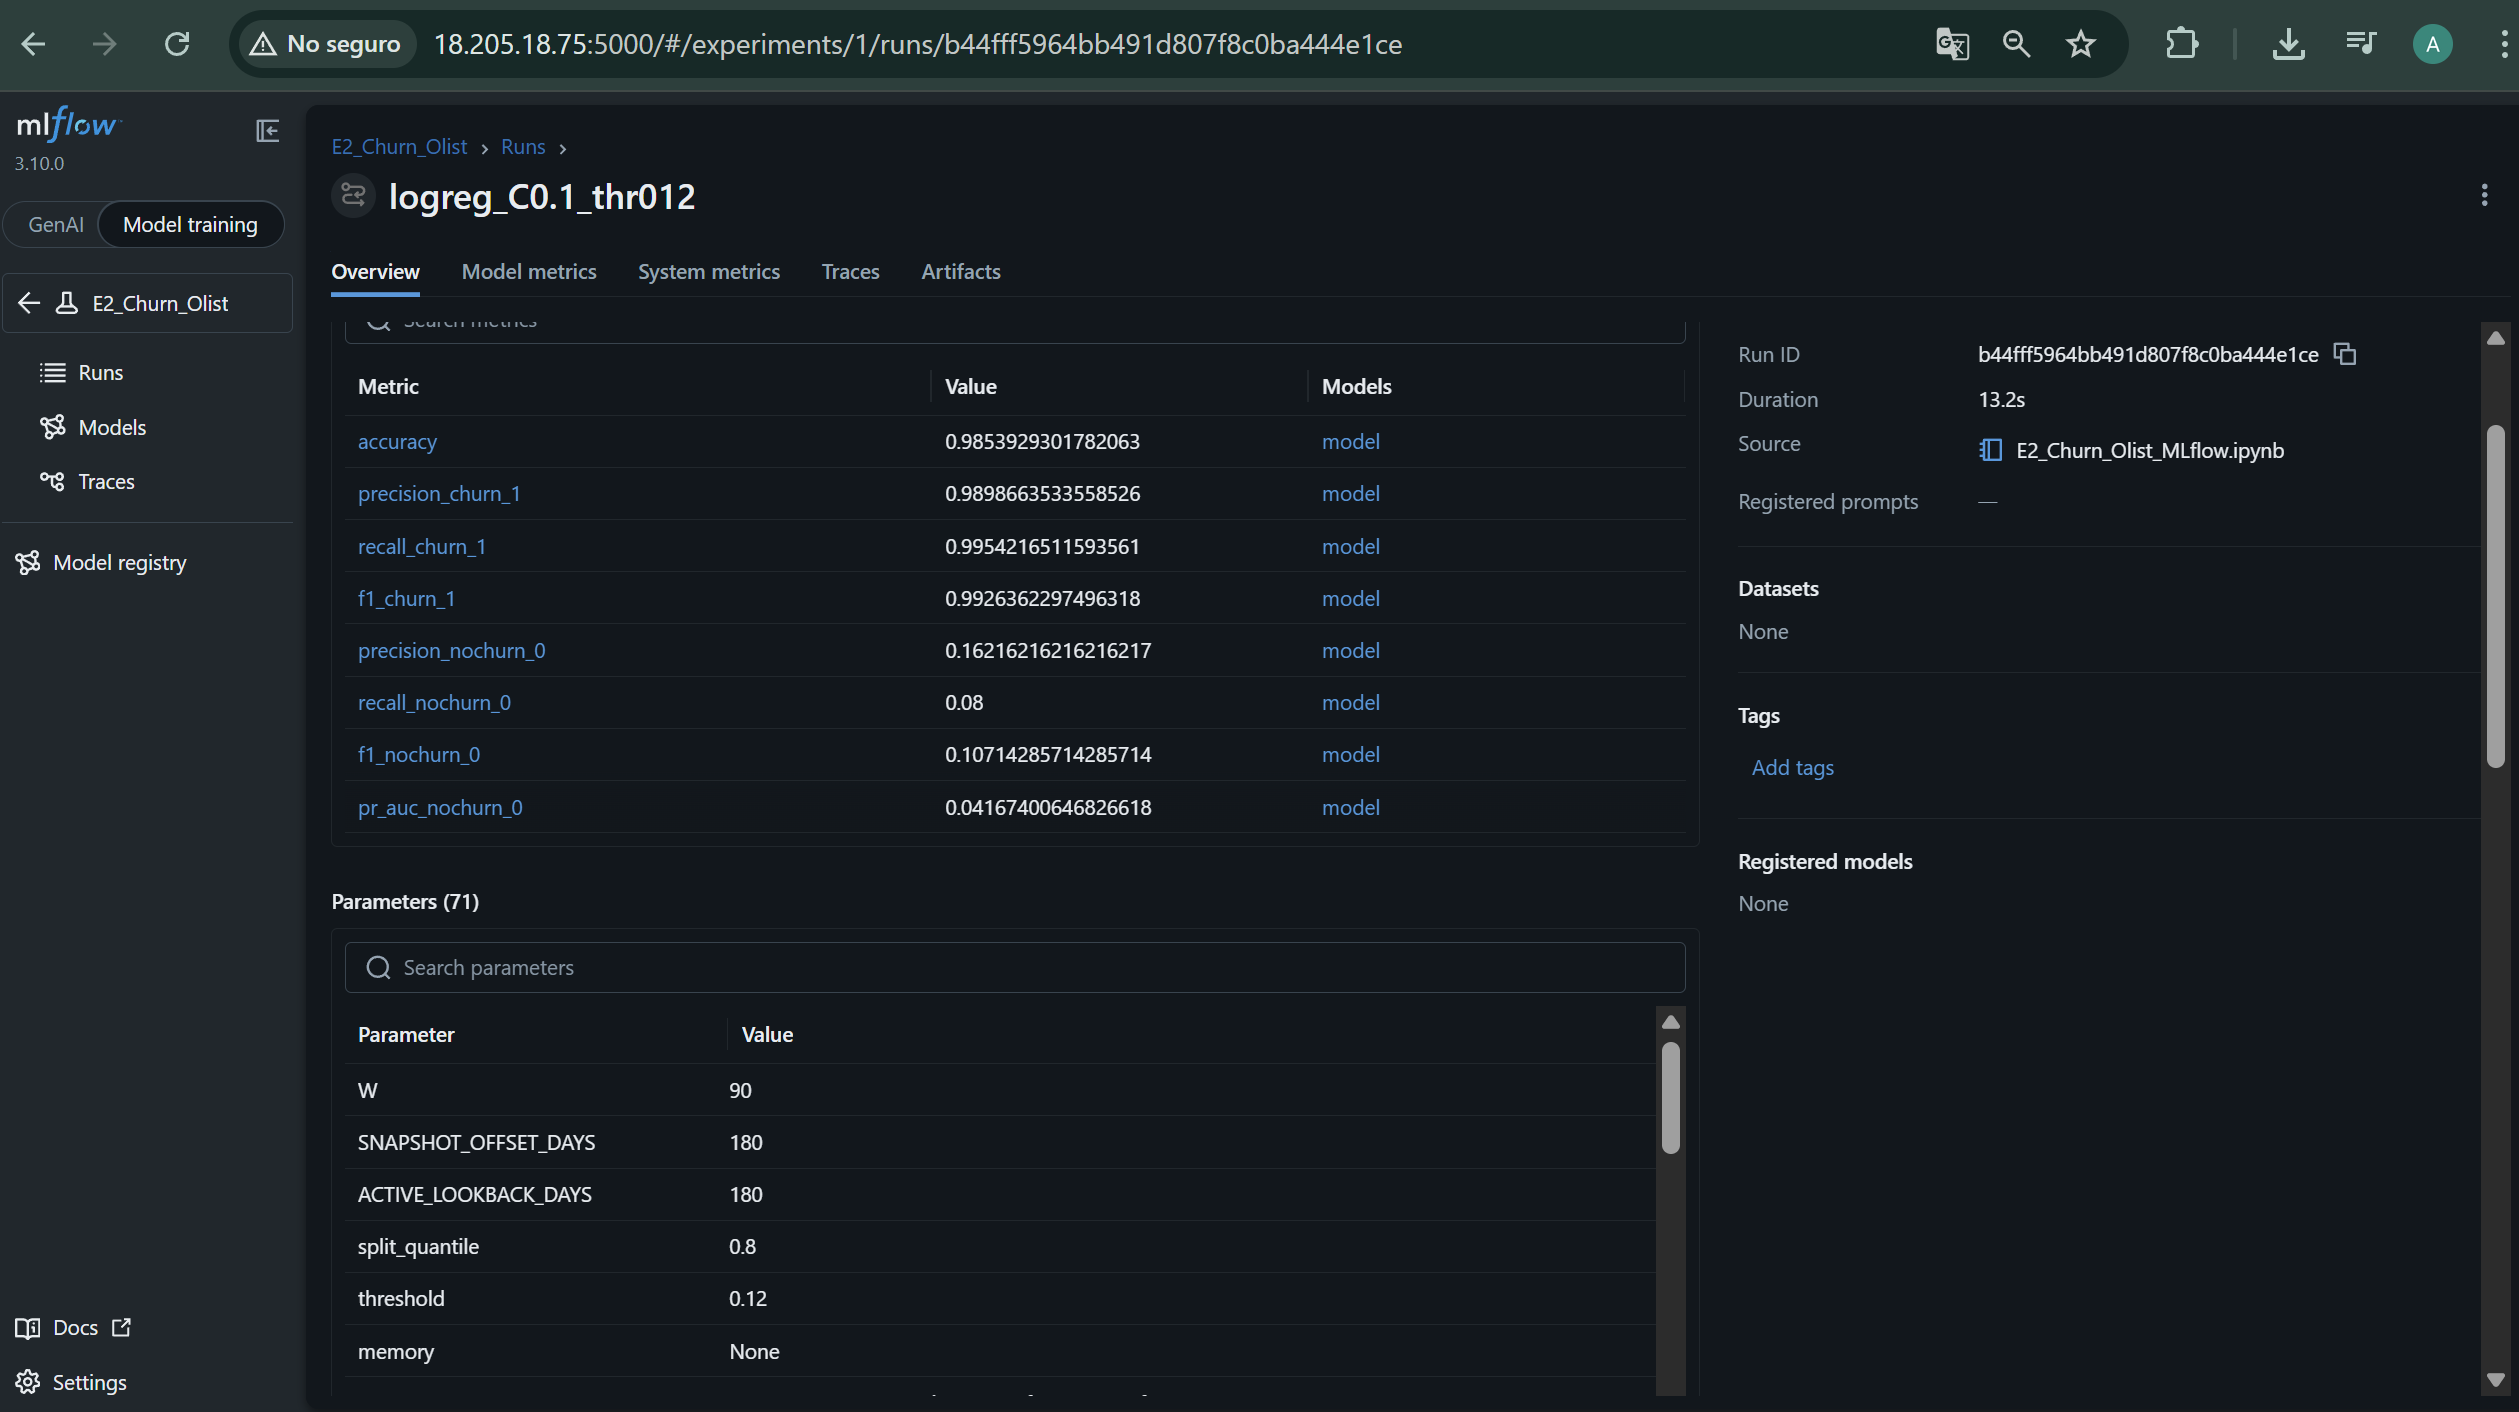
\includegraphics[width=\textwidth]{evidence/mlflow/EVID_MLFLOW_04_best_run_detail_params_metrics.png}
  \caption{Run ganador: parámetros y métricas.}
\end{subfigure}

\vspace{4pt}

\begin{subfigure}[b]{0.6\textwidth}
  \centering
  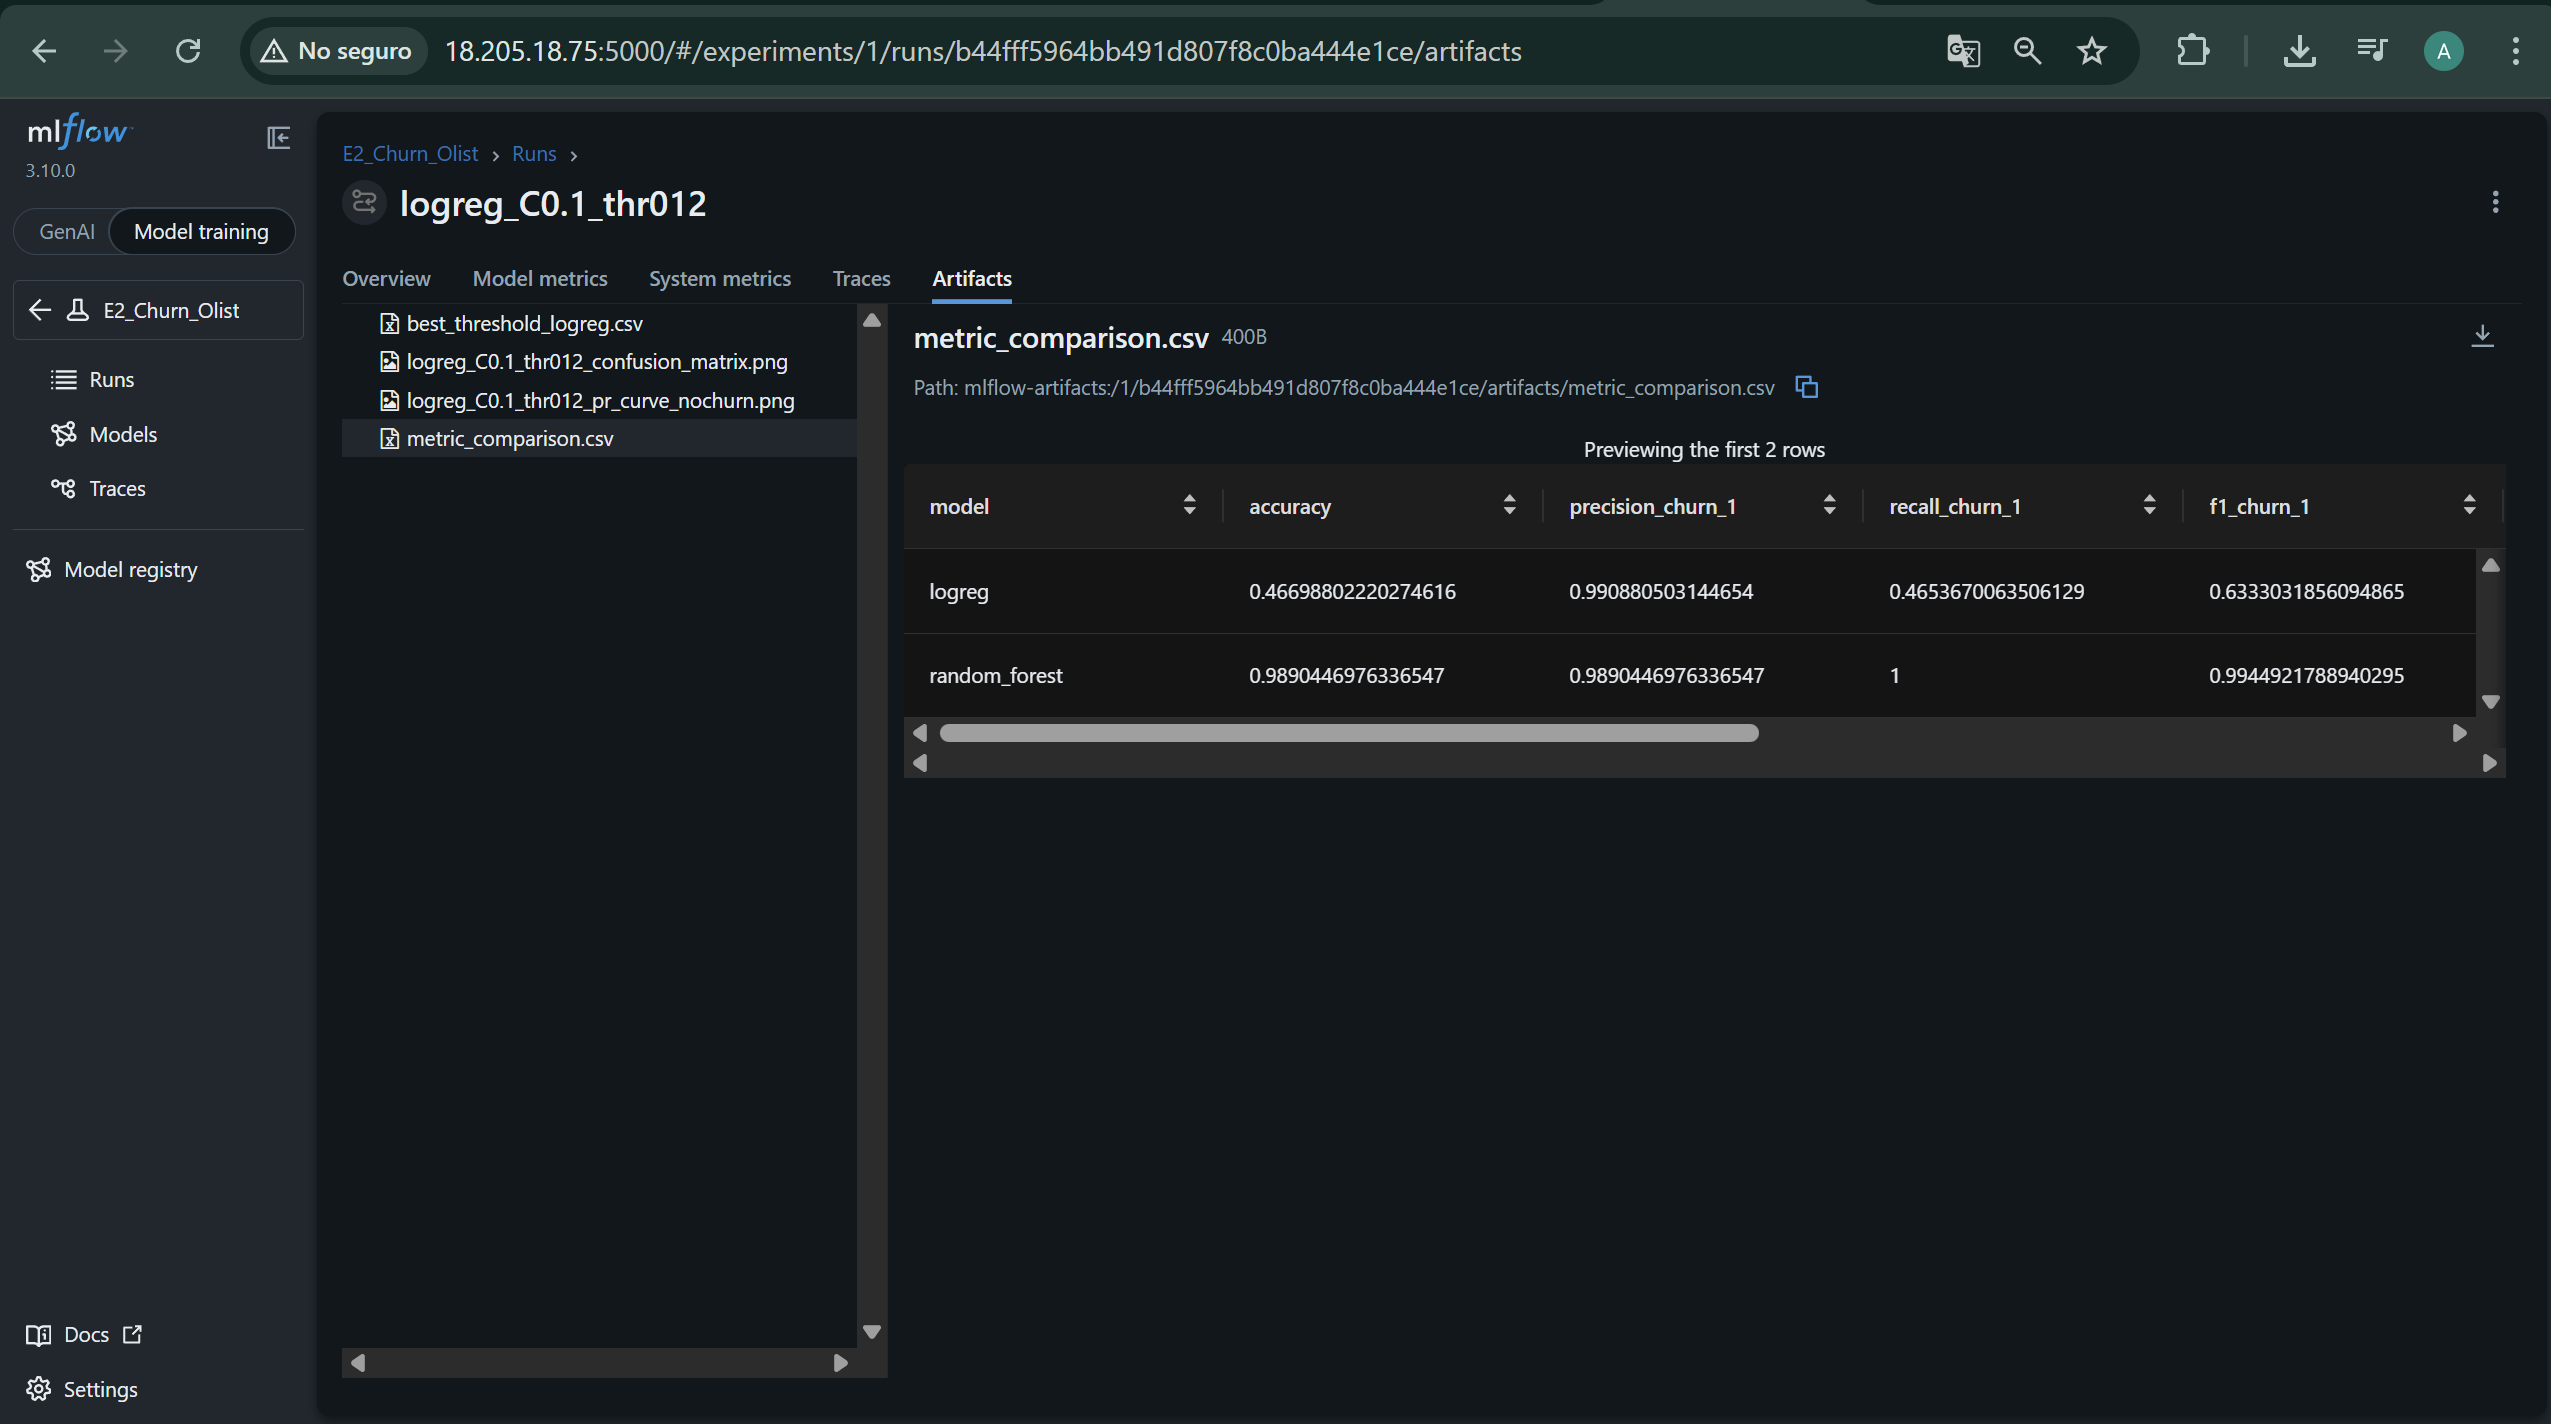
\includegraphics[width=\textwidth]{evidence/mlflow/EVID_MLFLOW_04_best_run_detail_artifacts.png}
  \caption{Run ganador: artefactos registrados.}
\end{subfigure}
\caption{MLflow: comparación y run ganador.}
\end{figure}

% ============================================================
\section{Tablero y API}

\subsection*{Arquitectura}

El producto final es un tablero de predicción individual accesible desde el
navegador, desplegado en la misma instancia EC2 con PM2 en el puerto 3000.
Consta de tres capas:

\begin{enumerate}[itemsep=2pt, topsep=2pt]
  \item \textbf{Frontend React/Vite}: formulario lateral que captura las 10
        variables del cliente y muestra el resultado.
  \item \textbf{API Express (Node.js)}: endpoint \texttt{POST /api/predict} que
        valida el payload, invoca Python vía \texttt{spawn} y devuelve JSON.
  \item \textbf{Inferencia Python}: \texttt{predict\_joblib.py} carga
        \texttt{best\_model\_logreg.joblib} y ejecuta \texttt{predict\_proba},
        retornando \texttt{churnProbability} $\in [0,1]$.
\end{enumerate}

\[
  \text{Usuario}
  \xrightarrow{\texttt{POST /api/predict}}
  \text{Express}
  \xrightarrow{\texttt{spawn}}
  \text{Python} \to \texttt{joblib}
  \xrightarrow{\texttt{churnProbability}}
  \text{Frontend}
\]

\subsection*{Variables de entrada}

\texttt{Recency}, \texttt{Frequency}, \texttt{Monetary},
\texttt{avg\_review\_score}, \texttt{avg\_delivery\_days},
\texttt{avg\_late\_days}, \texttt{avg\_num\_items}, \texttt{avg\_price\_sum},
\texttt{avg\_freight\_sum}, \texttt{customer\_state}.

\subsection*{Funcionalidades del tablero}

\begin{itemize}[itemsep=1pt, topsep=2pt]
  \item Predicción individual: probabilidad de churn en \%, nivel de riesgo
        (bajo / medio / alto) y probabilidad de retención complementaria.
  \item Panel de \textbf{contribución de features}: muestra las 8 variables con
        mayor impacto en la predicción, derivado directamente de los coeficientes
        del modelo, haciendo el resultado interpretable y accionable.
  \item Despliegue con \texttt{deploy\_churn\_dashboard.sh}: automatiza build
        Vite, creación de \texttt{.venv}, instalación de dependencias Python y
        arranque con PM2.
\end{itemize}

\begin{figure}[H]
\centering
\begin{subfigure}[b]{0.46\textwidth}
  
\includegraphics[width=\textwidth]{evidence/dashboard/EVID_DASH_01_prediction.png}
  \caption{Predicción individual con nivel de riesgo.}
\end{subfigure}
\hfill

\vspace{4pt}

\begin{subfigure}[b]{0.46\textwidth}
  
\includegraphics[width=\textwidth]{evidence/dashboard/EVID_DASH_02_macro.png}
  \caption{Visualizaciones macro del tablero.}
\end{subfigure}
\hfill
\begin{subfigure}[b]{0.46\textwidth}
  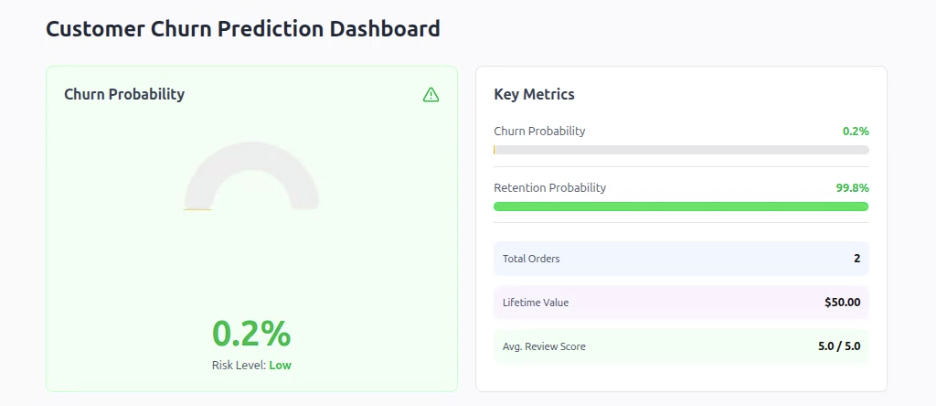
\includegraphics[width=\textwidth]{evidence/dashboard/EVID_DASH_0_churn.png}
  \caption{Distribución de churn en la población.}
\end{subfigure}
\caption{Tablero de predicción — vistas principales.}
\end{figure}

% ============================================================
\section{Video explicativo}

El video de presentación del proyecto (máx.\ 10 min) está disponible en el
siguiente enlace de Google Drive:

\begin{center}
  \url{https://drive.google.com/file/d/1YxZzugbef--xkANxXuvIvfrlS-3iVf4P/view?usp=sharing}
\end{center}

El video cubre: contexto del problema, definición del label, features y
partición temporal, modelos y evaluación, demostración del tablero y
principales conclusiones.

% ============================================================
\section{Conclusiones y trabajo futuro}

\begin{itemize}[itemsep=2pt, topsep=2pt]
  \item El dataset de Olist presenta desbalance extremo (recompra rara). El
        accuracy convencional no es una métrica válida; PR-AUC y $F_1$ para
        no-churn son las métricas relevantes.
  \item La Regresión Logística supera al Random Forest en la detección de
        recompra (PR-AUC 0.035 vs.\ 0.014). Su interpretabilidad vía coeficientes
        permite construir el panel de contribución de features sin herramientas
        adicionales.
  \item El ajuste del umbral de decisión ($\hat\tau=0.12$) incrementa
        $F_1^{(0)}$ de 0.025 a 0.113, demostrando que el calibrado del umbral
        tiene mayor impacto que la elección del algoritmo en datasets desbalanceados.
  \item MLflow en EC2 proporciona trazabilidad completa y reproducibilidad de
        los experimentos sin sobrecarga operativa significativa.
  \item El stack React/Vite + Express + Python + PM2 permite un despliegue
        reproducible y con gestión de ciclo de vida del proceso.
  \item \textbf{Trabajo futuro:} incorporar features por categoría de producto,
        explorar gradient boosting con calibración de probabilidades, y añadir
        monitoreo de deriva del modelo (\textit{data drift}) en producción.
\end{itemize}

% ============================================================
% TEAM REPORT — máximo 1 página adicional
% ============================================================
\newpage
\section*{Reporte de trabajo en equipo}
\addcontentsline{toc}{section}{Reporte de trabajo en equipo}

\hyphenpenalty=10000
\exhyphenpenalty=10000

{\small
\setlength{\tabcolsep}{4pt}
\renewcommand{\arraystretch}{2.2}

\begin{table}[H]
\centering
\caption*{Distribución de actividades — Entrega Final}
\begin{tabularx}{\textwidth}{
  >{\RaggedRight\arraybackslash}p{3.8cm}
  >{\RaggedRight\arraybackslash}p{2.8cm}
  >{\RaggedRight\arraybackslash}X
  >{\RaggedRight\arraybackslash}p{3.0cm}}
\toprule
\textbf{Miembro} & \textbf{Rol} & \textbf{Entregables} & \textbf{Evidencia} \\
\midrule
David Alan Delgado Zarco &
Modelado y metodología &
Label sin leakage, features (RFM + logística), split temporal, entrenamiento
LogReg/RF, barrido de umbral, joblib &
Commits en \texttt{E2\_Churn\_Olist\_MLflow.ipynb} y \texttt{outputs/} \\

Octavio Esquivel Alvarez del Castillo &
Reporte y QA &
LaTeX entrega final ($\leq$10 pág), integración de evidencias, revisión de
rúbrica, manuales de usuario e instalación &
Commits en \texttt{report/} \\

John Williams Morrill &
Tablero (React/Vite + API) &
Frontend React/Vite, API Express (\texttt{server/index.js}), panel de
contribución de features, script de despliegue &
Commits en \texttt{Tablero\_final/} \\

Jason Rosher Morrill &
MLOps / Infra (EC2 + MLflow) &
MLflow Tracking Server en EC2, runs con artefactos, PM2, capturas de
evidencia AWS/MLflow &
Commits en \texttt{server/} e \texttt{infra/}; capturas \texttt{evidence/aws}
y \texttt{evidence/mlflow} \\
\bottomrule
\end{tabularx}
\end{table}
}

\subsection*{Evidencia de commits en GitHub}

\begin{figure}[H]
\centering
\begin{subfigure}[b]{0.46\textwidth}
  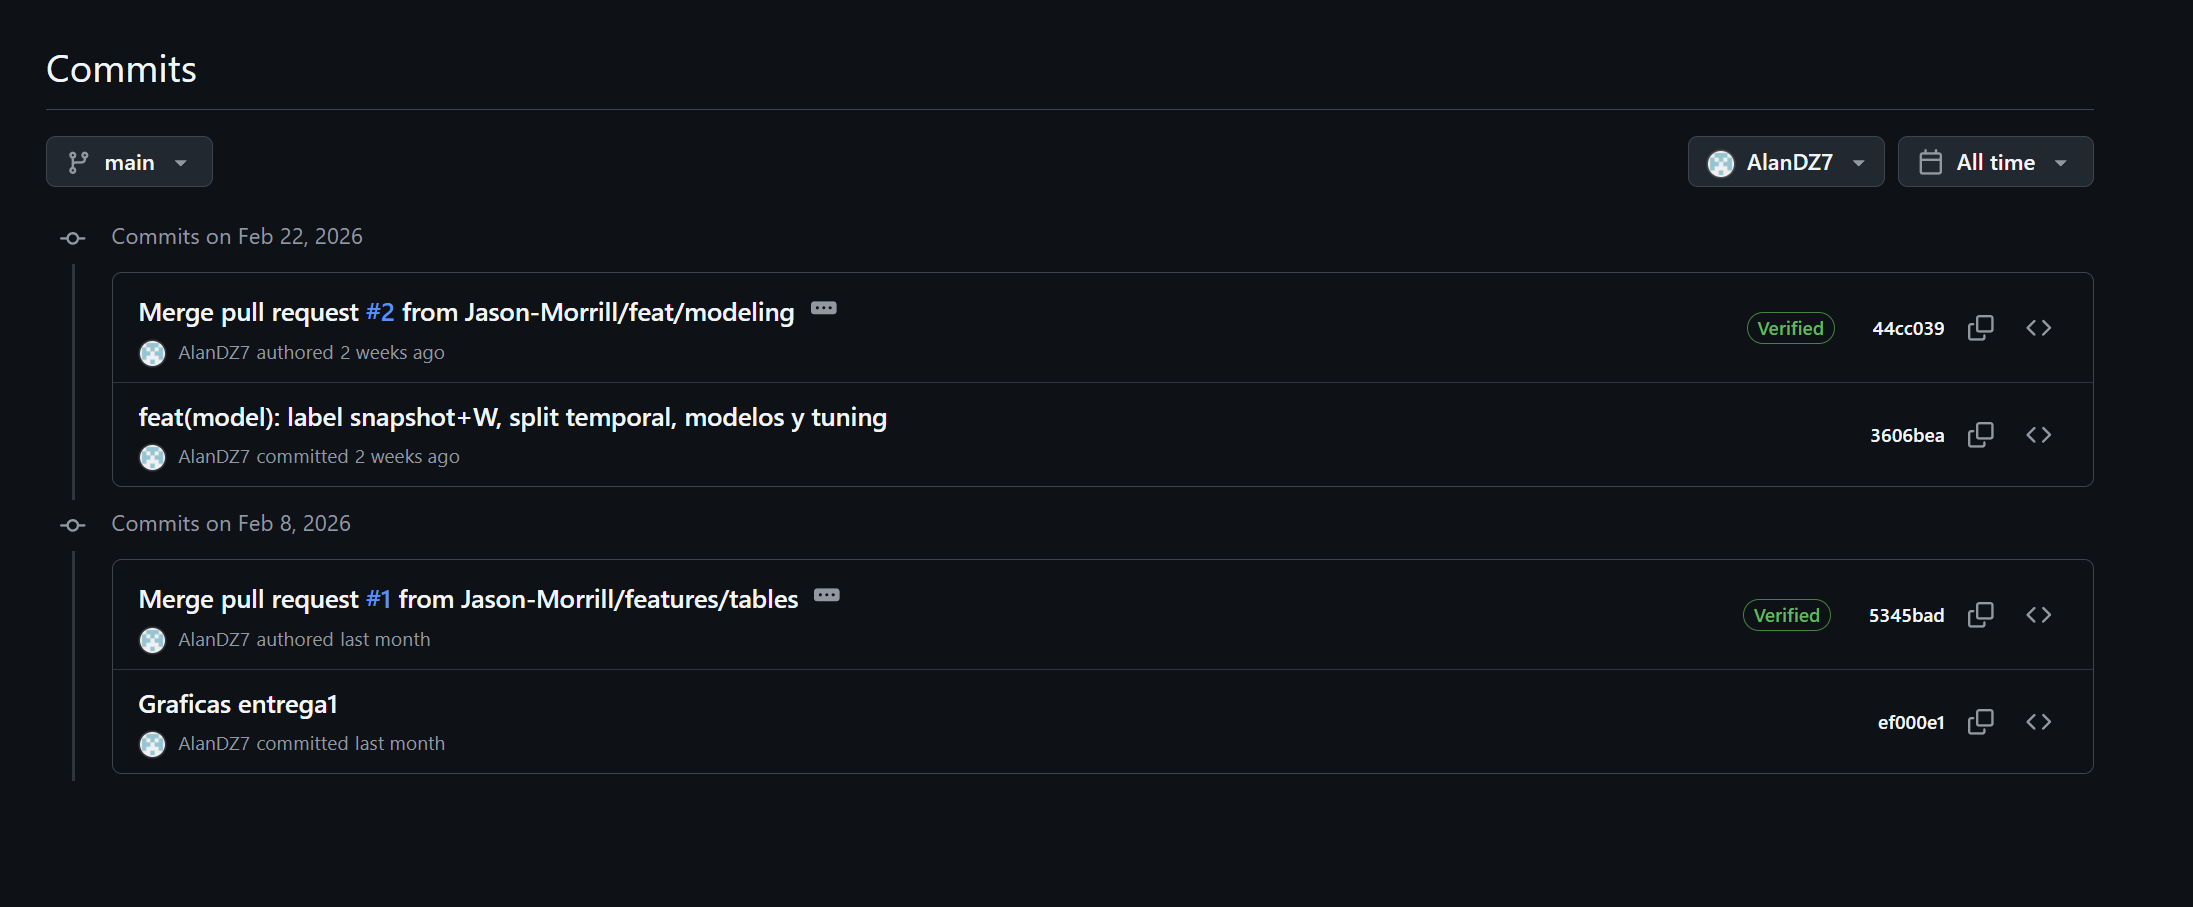
\includegraphics[width=\textwidth]{evidence/commits/EVID_COMMITS_01_david.png}
  \caption{Commits — David}
\end{subfigure}
\hfill
\begin{subfigure}[b]{0.46\textwidth}
  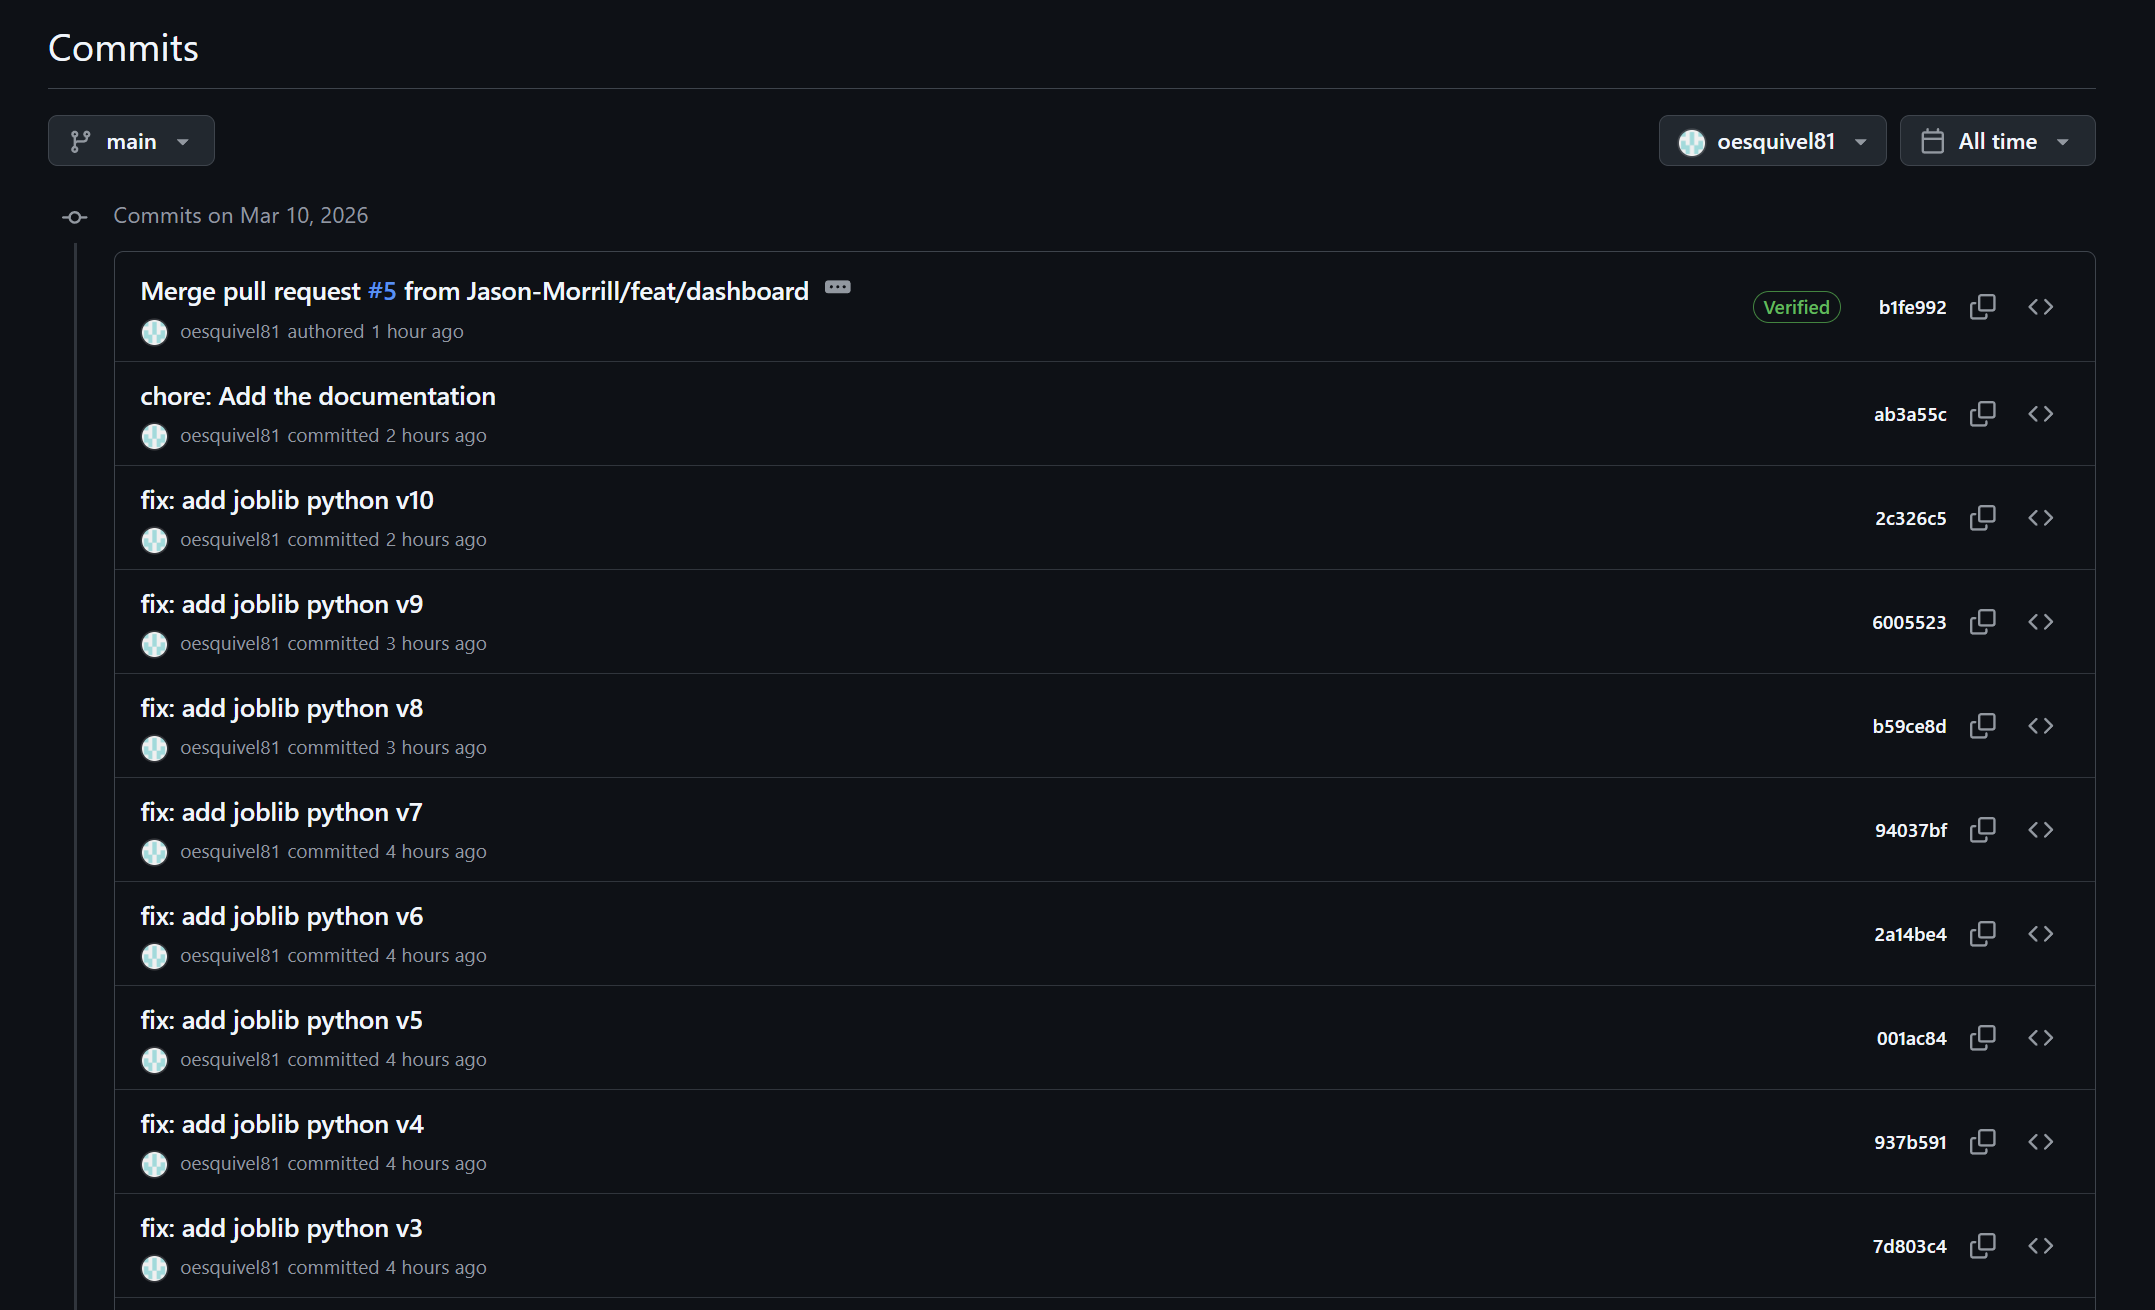
\includegraphics[width=\textwidth]{evidence/commits/EVID_COMMITS_02_octavio.png}
  \caption{Commits — Octavio}
\end{subfigure}

\vspace{6pt}

\begin{subfigure}[b]{0.46\textwidth}
  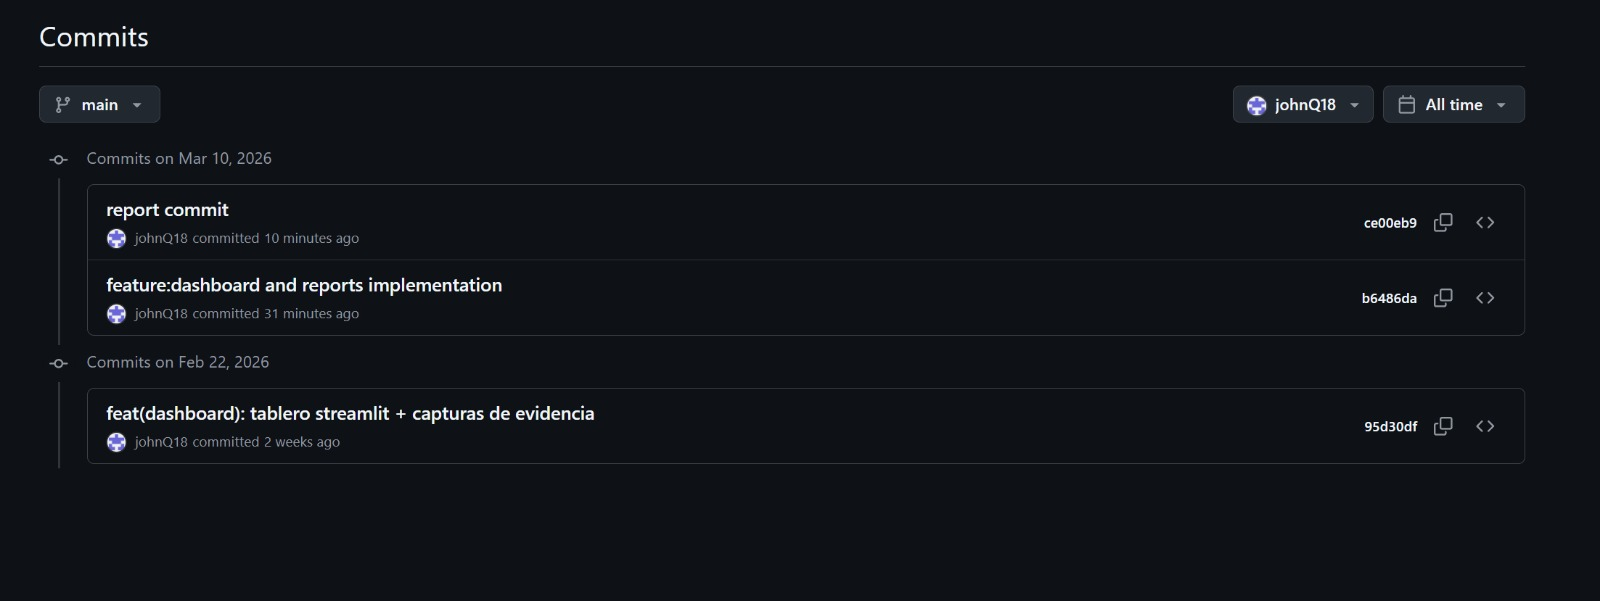
\includegraphics[width=\textwidth]{evidence/commits/EVID_COMMITS_03_john.jpeg}
  \caption{Commits — John}
\end{subfigure}
\hfill
\begin{subfigure}[b]{0.46\textwidth}
  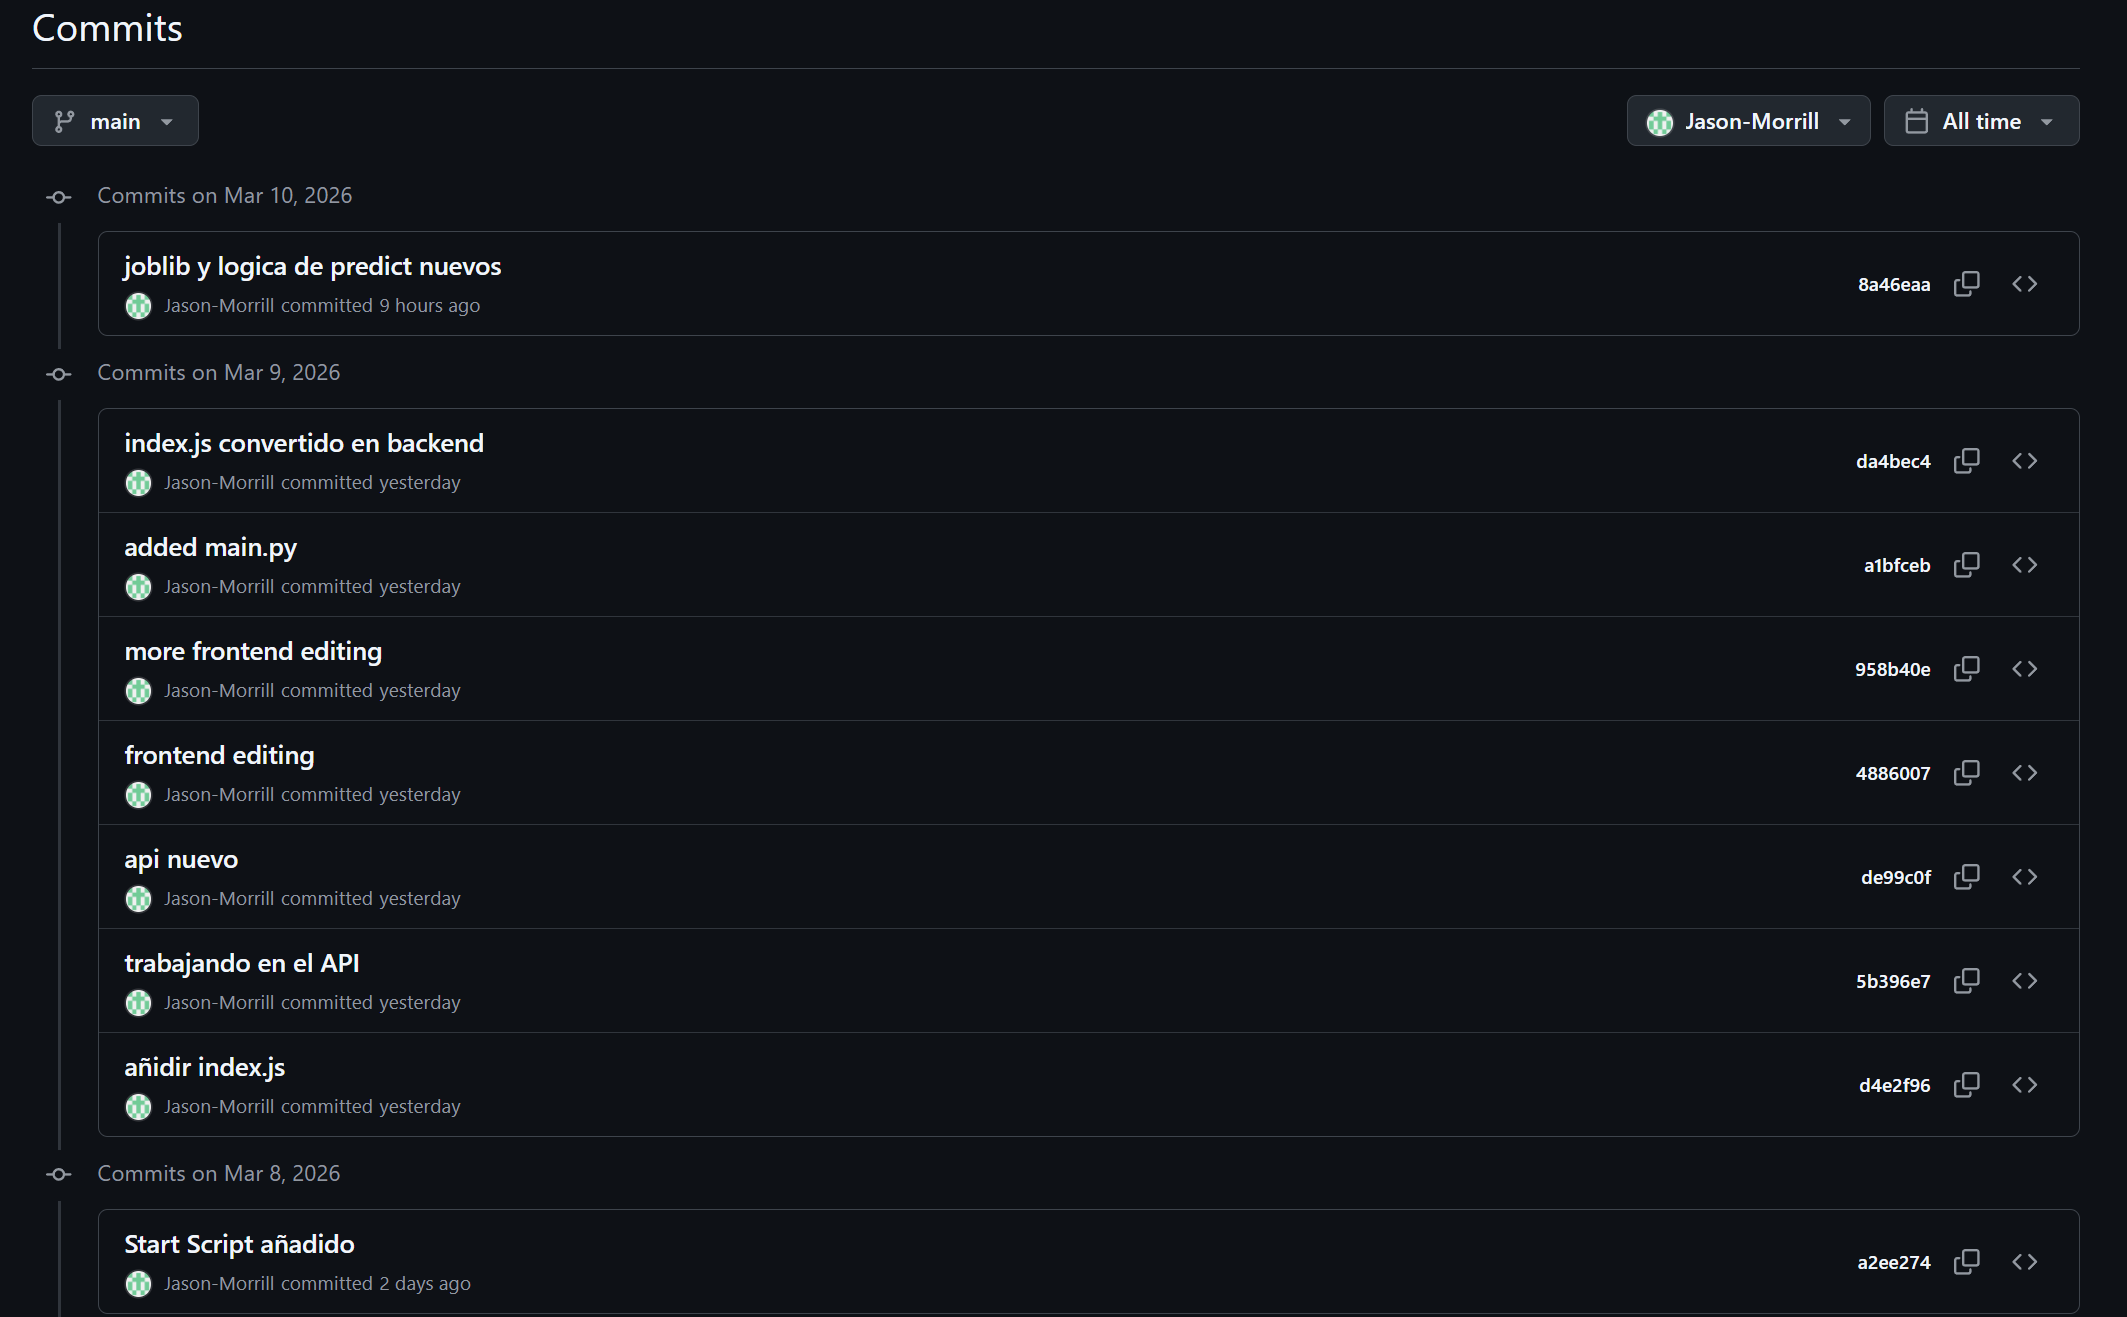
\includegraphics[width=\textwidth]{evidence/commits/EVID_COMMITS_04_jason.png}
  \caption{Commits — Jason}
\end{subfigure}
\caption{Evidencia de contribuciones individuales en el repositorio.}
\end{figure}

\end{document}
